\documentclass{article}

%Para usar idioma español
\usepackage[spanish]{babel}
%Codificación de teclado: en windows, pueden usar utf8 o, si su editor de texto no lo soporta, latin1. Ejemplo:
%usepackage[latin1]{inputenc}

\usepackage[utf8]{inputenc}
%\usepackage{amsmath}
%\usepackage{graphicx}
%Para posicionar las imágenes
\usepackage{float}
%Para encabezados personalizados
\usepackage{fancyhdr}
%Para tablas de más de una hoja
%\usepackage{longtable}
%Para incluir documentos en pdf
\usepackage{pdfpages}

%Utilizar links, pero sin colores
\usepackage{hyperref}
\hypersetup{
    colorlinks,%
    citecolor=black,%
    filecolor=black,%
    linkcolor=black,%
    urlcolor=black
}

%Definir márgenes
\oddsidemargin .1cm
\textwidth 15cm
\topmargin 0in
\textheight 8.5in


%Definir recta para encabezado y pie de página
\renewcommand{\headrulewidth}{0pt}
\renewcommand{\footrulewidth}{0.4pt}

\date{Marzo de 2012}

%Encabezado y pie de página
\pagestyle{fancy}
\rhead{Autor 1, Autor 2, Autor 3}
\lfoot{Problema nro. 1}
\cfoot{86.29 Prpoagación y Sistemas Irradiantes}
\rfoot{Página \textbf{\thepage}}







%COMIENZO DEL DOCUMENTO:
\begin{document}
\headheight 0cm
\graphicspath{{./img/}}

% Puede incorporarse un archivo .tex desde otro lugar, para que el documento quede más ordenado.
% Haremos esto para incluir la página del título (abrirlo para modificarlo).
\begin{titlepage}

\begin{center}



\includegraphics[scale=1]{img/fiuba.png} \\[1cm] 
%
\includegraphics[width=0.5\textwidth]{fiuba}\\[1cm]    

\textsc{\LARGE Facultad de Ingeniería - U.B.A.}\\[1.5cm]

\textsc{\Large 86.29 Propagación y Sistemas Irradiantes}\\[2cm]


% Título
{ \huge \bfseries Problema nro. 1:}\\
{ \huge \bfseries Dipolo Corto}\\[3cm]


\begin{flushleft} \large
\emph{Autores:}\\[.2cm]
\end{flushleft}
\begin{tabbing}
Fernando J. Iglesias \hspace{4cm}\= 94842\\
\end{tabbing}

\begin{flushleft} \large
\emph{Docentes:}\\[.2cm]
\end{flushleft}
Gustavo Fano\\
Pablo Lannes\\[.5cm]


\vfill

% Bottom of the page
%{\large \today}

\end{center}

\end{titlepage}

\clearpage
\tableofcontents
\clearpage

%Comando para crear una sección:
\section{Introducción}

Este breve documento muestra el uso de \LaTeX{} en la creación de informes para la materia 66.82 Propagación y Sistemas Irradiantes.

Se recomienda fuertemente la utilización de \LaTeX{} para las entregas. De utilizar otro formato, es necesario respetar igualmente todas las normas indicadas en este documento y enviar los informes convertidos a formato PDF.

\subsection{Ejemplo de subsección}

Texto en una subsección.

Para un párrafo nuevo, dejar un renglón en blanco en el \texttt{.tex}.\\

Para dejar una línea en blanco entre el texto, colocar dos barras invertidas (\verb|\\|). %Nota: el comando \verb se usa aquí para poder mostrar comandos de LaTeX en el pdf.

\subsubsection{Ejemplo de subsubsección: modo matemático}

Texto en una subsubsección.

Para escribir en modo matemático, puede usarse \verb|\[ ..... \]| o bien escribir \verb|$ .... $|. La primera opción es para escribir una ecuación en todo el renglón:

\[
 v(z,t) = e^{i \omega t} [V_+ e^{-i \gamma z} + V_- e^{i \gamma z}] =
 V_+ e^{i \omega t}[ e^{-i \gamma z} + \rho_L e^{i \gamma z}]
\]

La segunda opción es para escribir en medio del texto, por ejemplo $\varphi = 25$.

Recordar siempre colocar las unidades entre corchetes, por ejemplo $E = 30$ dBm o bien:

\[
E = 30 \ \mbox{dBm}				%La barra (\) es para crear una mayor separación.
\]

\section{Instalación}

El compilador de \LaTeX{} para MS Windows se llama MiKTeX y puede bajarse de la página \url{http://miktex.org/2.9/setup}.

En Linux hay que instalar los paquetes texlive y algunos más.

La escritura puede simplificarse con editores como Texmaker, Led, etc. Existen para Windows y para Linux. Más info en \url{http://en.wikipedia.org/wiki/Comparison_of_TeX_editors}.

\subsection{Paquetes}

Algunos de los paquetes usados en el preámbulo (antes de \verb|\begin{document}|) pueden no estar incluídos previamente en el compilador. En ese caso, deben descargarse, ya sea desde MiKTeX (MS Windows) utilizando el \texttt{Package Manager} o bien desde los repositorios correspondientes (Linux).

\section{Secciones de los informes de trabajos prácticos}

Los informes deben contar (al menos) con las siguientes secciones:

\begin{itemize}
 \item Objetivos
 \item Desarrollo (donde se resuelven las tareas de los enunciados, que \emph{también deben estar presentes aquí})
 \item Conclusiones
 \item Referencias
 \item Anexos (si fueran necesarios)
\end{itemize}

\section{Gráficos}

Los gráficos siempre deben presentarse con escalas adecuadas, y deben contar con las siguientes características:

%Bloque para describir distintos items:
\begin{itemize}
 \item Magnitud graficada y unidad (entre corchetes) en ambos ejes.
 \item Grilla (comando \texttt{grid on}).
 \item Siempre que se requiera comparar resultados, es conveniente hacerlo en el mismo gráfico, para poder ver las diferencias más fácilmente. Para graficar múltiples curvas en un gráfico utilizar, por ejemplo, el comando \texttt{hold on}.
 \item Cuando haya más de un trazo en el mismo gráfico, agregar leyendas adecuadas para su correcta diferenciación. Utilizar el comando \texttt{legend}.
 \item Para visualizar el eje $x$ en escala logarítmica, utilizar el comando \texttt{semilogx}.
\end{itemize}

Por ejemplo:

\begin{figure}[H]	%inicia el entorno para insertar una imagen
 \centering			%centra la imagen en la página
 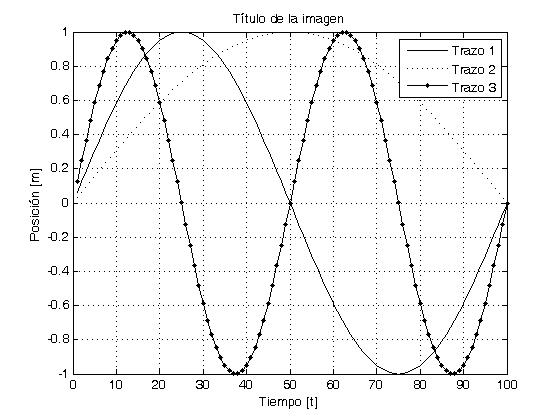
\includegraphics[width = 10cm]{grafico_matlab}	%insertar la imagen; en vez de width puede usarse height o scale
 %LA IMAGEN PUEDE SER JPG, PNG, PDF, ETC.
 \caption{Sistema de referencia en una línea de transmisión.}	%Descripción de la imagen
 \label{figura1}
\end{figure}

Para referenciar una figura, utilizar el comando \verb|\ref{}|. Por ejemplo, ver la Figura \ref{figura1}.

\section{Añadir Anexos}

Pueden incluirse Anexos como \textit{listings} de \texttt{Matlab}, por ejemplo, ver Anexo \ref{matlab_ej1} con el listado de Matlab para producir la Figura \ref{figura1}. %El comando \ref{} funciona en conjunto con el comando \label{}, para referenciar secciones, subsecciones, imágenes, tablas, etc.



\section{Tablas}

Las tablas en \LaTeX{} pueden realizarse de la siguiente manera:

\begin{table}[H]
\centering
\begin{tabular}{|c|c|c|}	%alineación centrada
\hline
AAA & BBB & CCC\\
\hline
D & E & F\\
\hline
G & H & I\\
\hline
\end{tabular}
\caption{Primera tabla}	%Opcional
\label{tabla1}			%Opcional
\end{table}

También puede cambiarse la alineación y los bordes:

\begin{table}[H]
\centering
\begin{tabular}{||l|c|r||}	%%alineación izquierda, centrada y derecha
\hline
AAA & BBB & CCC\\
\hline
\hline
D & E & F\\
\hline
G & H & I\\
\hline
\end{tabular}
\caption{Segunda tabla}	%Opcional
\label{tabla2}			%Opcional
\end{table}

\section{Ejemplo: Línea Cargada}

\begin{figure}[H]	%inicia el entorno para insertar una imagen
 \centering			%centra la imagen en la página
 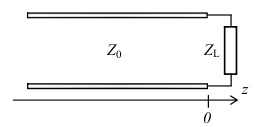
\includegraphics[width = 8cm]{linea_sist_ref1}	%insertar la imagen; en vez de width puede usarse height o scale
 \caption{Sistema de referencia en una línea de transmisión.}	%Descripción de la imagen
 \label{figura2}
\end{figure}

Observar la Figura \ref{figura2}. %Referencia a una imagen en el texto.

Tensiones y corrientes en la línea

\[
 v(z,t) = e^{i \omega t} [V_+ e^{-i \gamma z} + V_- e^{i \gamma z}] =
 V_+ e^{i \omega t}[ e^{-i \gamma z} + \rho_L e^{i \gamma z}]
\]

\[
 i(z,t) = \frac{e^{i \omega t}}{Z_0} [V_+ e^{-i \gamma z} - V_- e^{i \gamma z}] =
 \frac{V_+}{Z_0} e^{i \omega t}[ e^{-i \gamma z} - \rho_L e^{i \gamma z}]
\]

Donde:
\[
 \gamma = \beta - i \ \alpha
\]

Por lo que:

\[
 v(z,t) = v_0 \ e^{-\alpha z} \  e^{i (\omega t - \beta z)} 
\]

De donde reconocemos que la velocidad de propagación de la onda es:
\[
 c = \frac{\omega}{\beta} \longrightarrow \beta = \frac{\omega}{c} = \frac{2 \pi f}{\lambda f} = \frac{2 \pi}{\lambda}
\]


Coeficiente de reflexión en la carga ($z=0$)

\[
 \rho_L = \frac{V_-}{V_+}= \frac{Z_L - Z_0}{Z_L+Z_0}
\]

Coeficiente de transmisión en la carga ($z=0$)

\[
 \tau_L=\frac{V_L}{V_+}= 1+\rho = \frac{2 Z_L}{Z_L+Z_0}
\]


Return Loss

\[
 RL = -20 \log(|\rho|)
\]

Impedancia y admitancia en la línea

\[
 Z(z) = \frac{v(z,t)}{i(z,t)} =
 Z_0 \frac{ e^{-i \gamma z} + \rho_L e^{i \gamma z} }{ e^{-i \gamma z} - \rho_L e^{i \gamma z} }=
 Z_0 \frac{ 1 + \rho_L e^{2 i \gamma z} }{ 1 - \rho_L e^{2 i \gamma z} }=
 Z_0 \frac{Z_L \cos(\gamma z) - i Z_0 \sin(\gamma z)}{Z_0 \cos(\gamma z) - i Z_L \sin(\gamma z)} =
 Z_0 \frac{Z_L  - i Z_0 \tan(\gamma z)}{Z_0 - i Z_L \tan(\gamma z)}
\]

\[
 Y(z) = \frac{i(z,t)}{v(z,t)} =
 Y_0 \frac{Y_L \cos(\gamma z) - i Y_0 \sin(\gamma z)}{Y_0 \cos(\gamma z) - i Y_L \sin(\gamma z)} =
 Y_0 \frac{Y_L - i Y_0 \tan(\gamma z)}{Y_0 - i Y_L \tan(\gamma z)}
\]

Relación de onda estacionaria (SWR)

\[
 ROE = \frac{V_M}{V_m} = \frac{1+|\rho|}{1-|\rho|}
\]

Línea con generador

\begin{figure}[H]
 \centering
 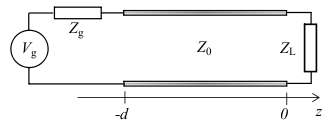
\includegraphics[width = 8cm]{linea_generador_y_carga} %ver que acá la Figura no tiene label ni caption. Por lo tanto, no puede ser referenciada.
\end{figure}

\[
 V_+ = \frac{ Z_0 (Z_L+Z_0) }
{(Z_L + Z_0)(Z_g+Z_0) e^{i k d} + (Z_L - Z_0)(Z_0-Z_g)e^{-i k d} } V_g
\]

\[
 V_-=\rho V_+
\]



%Apéndices o anexos a partir de aquí:
\appendix

\section{Código de Matlab/Octave, Ejercicio 1}
\label{matlab_ej1}

Pueden incluirse los listados de Matlab/Octave mediante los comandos:

\verb| \begin{verbatim} ...código...  \end{verbatim} |\\
 
Por ejemplo:

\begin{verbatim}
clc
clear all
close all
x = [1:100];
y1 = sin(2*pi*x/1e2);
y2 = sin(2*pi*x/2e2);
y3 = sin(2*pi*x/.5e2);

figure
plot(x,y1,'k')
hold on
plot(x,y2,'k:')
plot(x,y3,'k.-')
xlabel('Tiempo [t]')
ylabel('Posición [m]')
title('Título de la imagen')
legend('Trazo 1','Trazo 2','Trazo 3')
grid on
\end{verbatim}



\end{document}
